\newpage
\chapter{Estudio espectral de los polinomios discretos de Legendre}

No es difícil convencerse de que las condiciones de ortogonalidad
impuestas en la definición de la base de Legendre discreta
$\cali{L}^{n}$
forzan a las entradas de los polinomios discretos $\cali{L}^{n,k}$
a cambiar más frecuentemente de signo conforme aumenta
el grado $k$, luego, conforme $k$ tiende a $n-1$,
la cantidad de oscilaciones aumenta; revisemos, 
por ejemplo, el caso $n=4$.

\begin{minipage}{0.5\textwidth}
\begin{figure}[H]
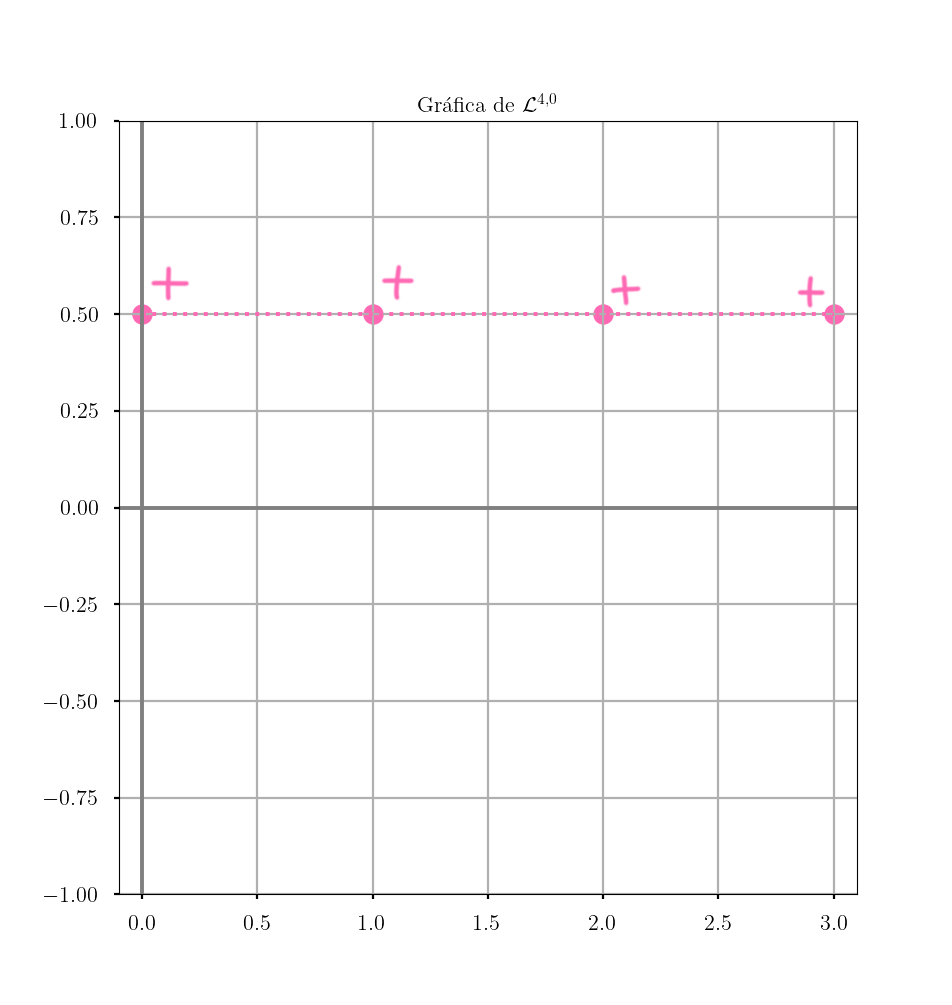
\includegraphics[scale=0.3]{oscil1}
\end{figure}
\end{minipage} \hfill
\begin{minipage}{0.45\textwidth}
1.- Por definición,

\[
\cali{L}^{4,0} = \left(
\frac{1}{2}, \frac{1}{2}, \frac{1}{2}, \frac{1}{2}
\right).
\]
\end{minipage}


\begin{minipage}{0.5\textwidth}
2.- La señal $\cali{L}^{4,1} \in \IR^{4}$ es un polinomio discreto de
dimensión 4 y grado 1 que se obtiene exigiendo las
siguientes condiciones

\[
\langle \cali{L}^{4,1} , \cali{L}^{4,0} \rangle=0
\hspace{0.2cm} \text{y} \hspace{0.2cm}
\langle \cali{L}^{4,1} , \cali{L}^{4,1} \rangle=1;
\]
esta primera condición se refleja en que 
las alturas de los puntos de la gráfica de 
$\cali{L}^{4,1}$ deben sumar cero;
esto implica un cambio de signo (y sólo uno,
pues el polinomio es lineal).

\end{minipage} \hfill
\begin{minipage}{0.45\textwidth}
\begin{figure}[H]
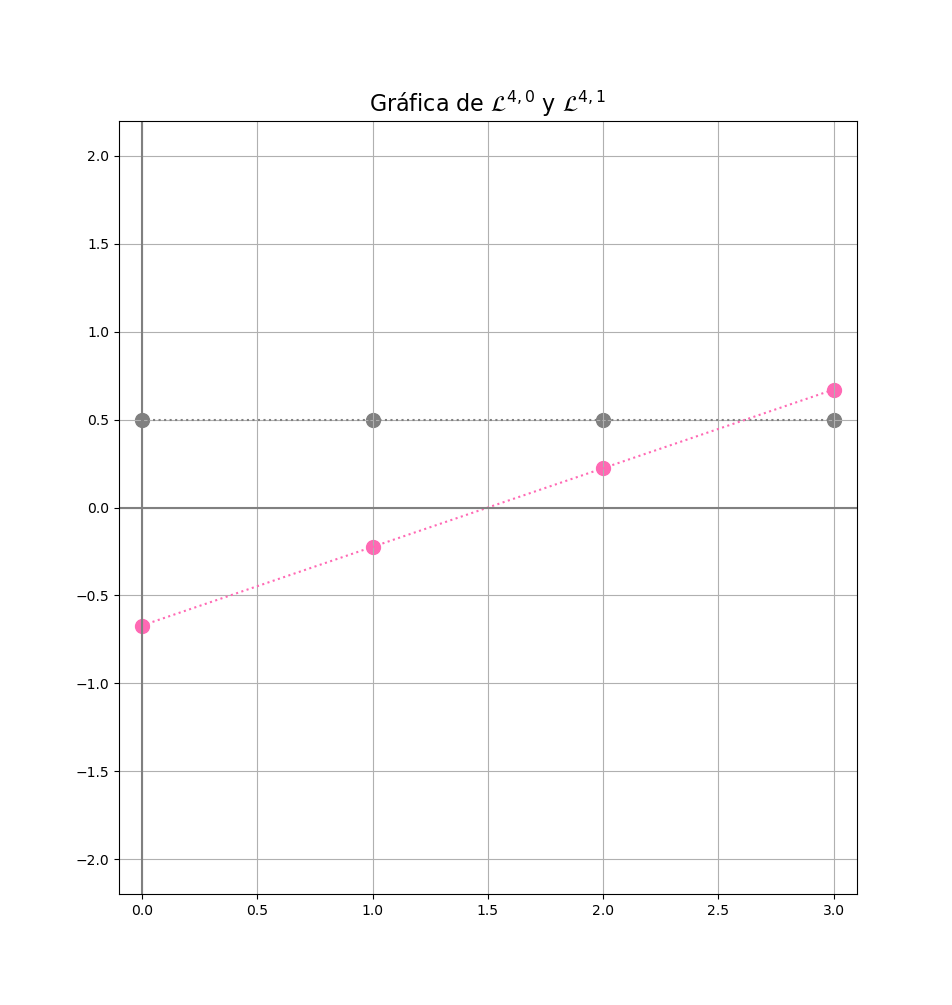
\includegraphics[scale=0.3]{oscil2}
\end{figure}
\end{minipage}

\noindent
3.- Las condiciones de la definición
de $\cali{L}^{4,2} \in \IR^{4}$ son

\[
\langle \cali{L}^{4,2} , \cali{L}^{4,0} \rangle=0,
\hspace{0.2cm}
\langle \cali{L}^{4,2} , \cali{L}^{4,1} \rangle=0,
\hspace{0.2cm} \text{y} \hspace{0.2cm}
\langle \cali{L}^{4,2} , \cali{L}^{4,2} \rangle=1;
\]
observe que si las entradas de 
$\cali{L}^{4,2}$ fuesen todas positivas o todas negativas,
entonces no se tendría la ortogonalidad
con la señal constante $\cali{L}^{4,0}$.


\begin{figure}[H]
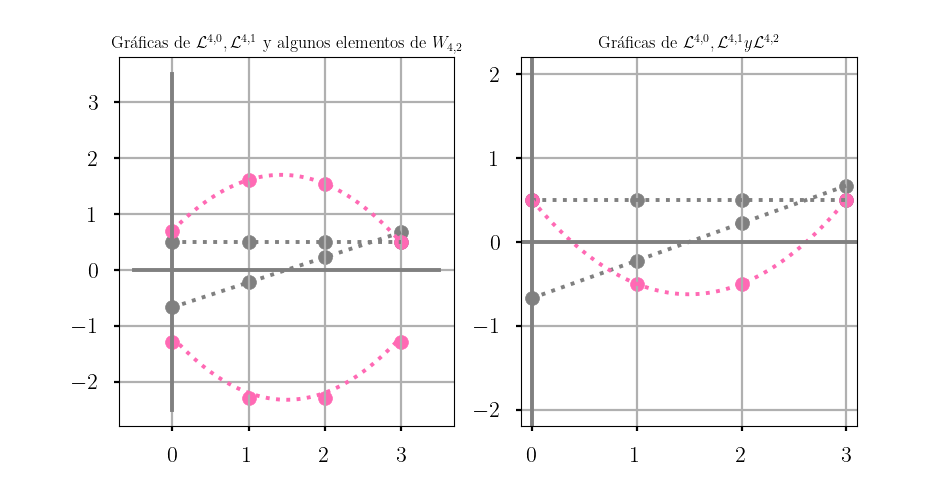
\includegraphics[scale=0.3]{oscil3}
\end{figure}

4.- 
\begin{figure}[H]
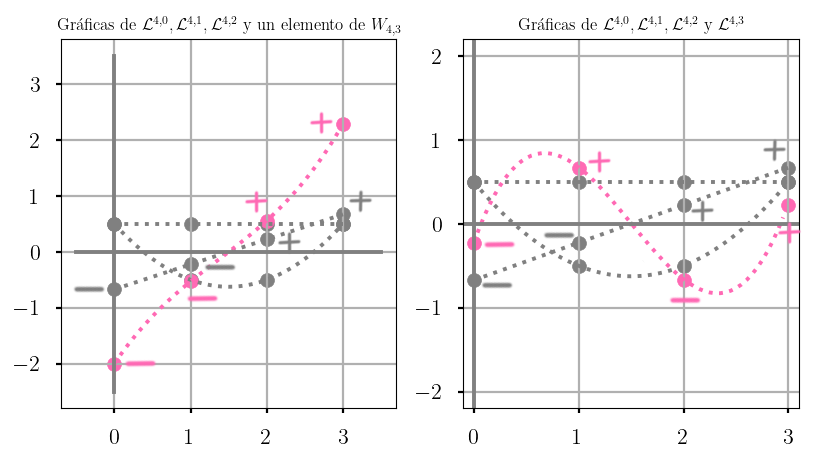
\includegraphics[scale=0.3]{oscil4}
\end{figure}



\subsection{Estudio de presencia de frecuencias particulares via mediciones de distancia a espacios de frecuencia}

Queremos ahora generalizar el estudio anterior y no restringirnos
al estudio de frecuencias enteras, \TODO{Aquí dí por qué}
sino el poder elegir una frecuencia $\omega \geq 0$ respecto
a la cual comparar a la señal. A pesar
de que ya no contaremos con la seguridad de trabajar con bases
ortonormales de $\IR^{n}$, queremos considerar espacios de frecuencias
en base a los cuales medir la distancia de $x$ a estos, siendo
esta una medida de qué tanto reacciona $x$ a la frecuencia $\omega$.
\TODO{Cita el ejemplo en el que haces esto para medir qué tan afín es
una señal.}

\sidenote{Para simplificar la notación, denotamos por $I_{n}$ al intervalo
$\{ \frac{\mu }{n}  : 0 \leq \mu \leq n-1 \}$.}

\begin{defi}
Si $n \geq 2$ es un entero y $\omega \geq 0$ es un número no negativo
\TODO{y no múltiplo escalar de $n$}, entonces a los vectores

	\begin{equation}
	\label{eq5: 19Marzo}
	f_{n, \omega}= \left( \xi_{n, \omega} cos \left(2 \pi \omega \frac{\mu }{n} \right) \right)_{0 \leq \mu \leq N-1}
	\in \IR^{n}
	\end{equation}
y 

	\begin{equation}
	\label{eq6: 19Marzo}
	g_{n, \omega}= \left( \eta_{n, \omega} sen \left(2 \pi \omega \frac{\mu }{n}\right) \right)_{0 \leq \mu \leq N-1}
	\in \IR^{n},
	\end{equation}
donde

\begin{equation}
\label{eq7: 19Marzo}
\xi_{n, \omega}= 
\left\{
	\begin{array}{ll}
		\sqrt{2} \cdot \left( N + \frac{sen(2 \pi \omega)
	cos(2 \pi \omega \left( 1- \frac{1}{n} \right))}{sen \left(2 \pi 
	\frac{\omega}{n} \right)} \right)^{-\frac{1}{2}}  & \mbox{si } n \nmid \omega,  \\
		\frac{1}{\sqrt{n}} & \mbox{si } n \mid \omega,
	\end{array}
\right.
\end{equation}
y

	\begin{equation}
	\label{eq8: 19Marzo}
	\eta_{n, \omega}= \sqrt{2} \cdot \left( N - \frac{sen(2 \pi \omega)
	cos(2 \pi \omega \left( 1- \frac{1}{n} \right))}{sen \left(2 \pi 
	\frac{\omega}{n} \right)} \right)^{-\frac{1}{2}}
	\end{equation}

\noindent	
les llamaremos los \textbf{vectores base de frecuencia $\omega$}.
\TODO{$g_{n, \omega}$ es el vector cero cuando $\omega$ es múltiplo
de $n$. Por el momento, en lo que sigue sólo voy a considerar frecuencias
que no sean múltiplos de la dimensión.}
\end{defi}

Fijados $n$ y $\omega$,
el espacio que generan los vectores de frecuencia $\omega$
$f_{n, \omega}$ y $g_{n, \omega}$ es

\begin{align}
\label{eq2: 20Marzo}
P_{\omega}:= & span(f_{n, \omega}, g_{n, \omega}) \\ 
= &
\{ a \left( cos \left(2 \pi \omega t \right) \right)_{t \in I_{n}} +
b ( sen (2 \pi \omega t ))_{t \in I_{n}} : 
\hspace{0.2cm} a, b \in \IR \} \\ \nonumber
\end{align}

luego, $P$ es el plano que consiste de las señales
$n-$dimensionales de frecuencia (pura) $\omega$;
\sidenote{\TODO{Deberías poner esta definición más arriba}} 
en efecto, si $\phi$ es un desfase cualquiera, entonces,
por la regla del coseno de la suma,
\[
(cos (2 \pi \omega (t + \phi)))_{t \in I_{n}}
= a  (cos(2 \pi \omega t))_{t \in I_{n}} -
b  (sen(2 \pi \omega t))_{t \in I_{n}} \in P_{\omega},
\]
donde
$a:= cos(2 \pi \omega \phi)$ y $b= sen(2 \pi \omega \phi)$;
similarmente se deduce que todo vector de $\IR^{n}$ 
de la forma $(sin (2 \pi \omega (t + \phi)))_{t \in I_{n}}$
es elemento de $P_{\omega}$.



Es razonable pues
medir la cercanía de una señal $n-$dimensional $x \in \IR^{n}$
a tener frecuencia $\omega$
con el ángulo que $x$ forma con el plano $P_{\omega}$,
coseno que, según la proposición
\ref{prop: algunos hechos sobre el angulo entre un vector y un subespacio}
es
\begin{equation}
\label{eq0: 20Mar}
cos \left( \measuredangle (x, W) \right) = \frac{|| \Pi_{W}(x) ||}{||x||}
\in [0,1].
\end{equation}

\TODO{Por casualidad encontré la página de ``cosine similarity'' en wikipedia.
Habla de esta forma de medir similitudes en base a cosenos de ángulos. 
Deberías citarla.}

\begin{figure}[H]
	\sidecaption{
	Según la relación \eqref{eq0: 20Mar}, 
	si $\frac{||\Pi_{P_{\omega}}(x)}{||x||}$ es cercano 
	a uno (resp. a cero), entonces $x$ es muy parecido a una señal de frecuencia $\omega$
	(resp. se aleja de ser una señal de frecuencia $\omega$).
	\label{fig: 20Mar23_1}
	}
	\centering
	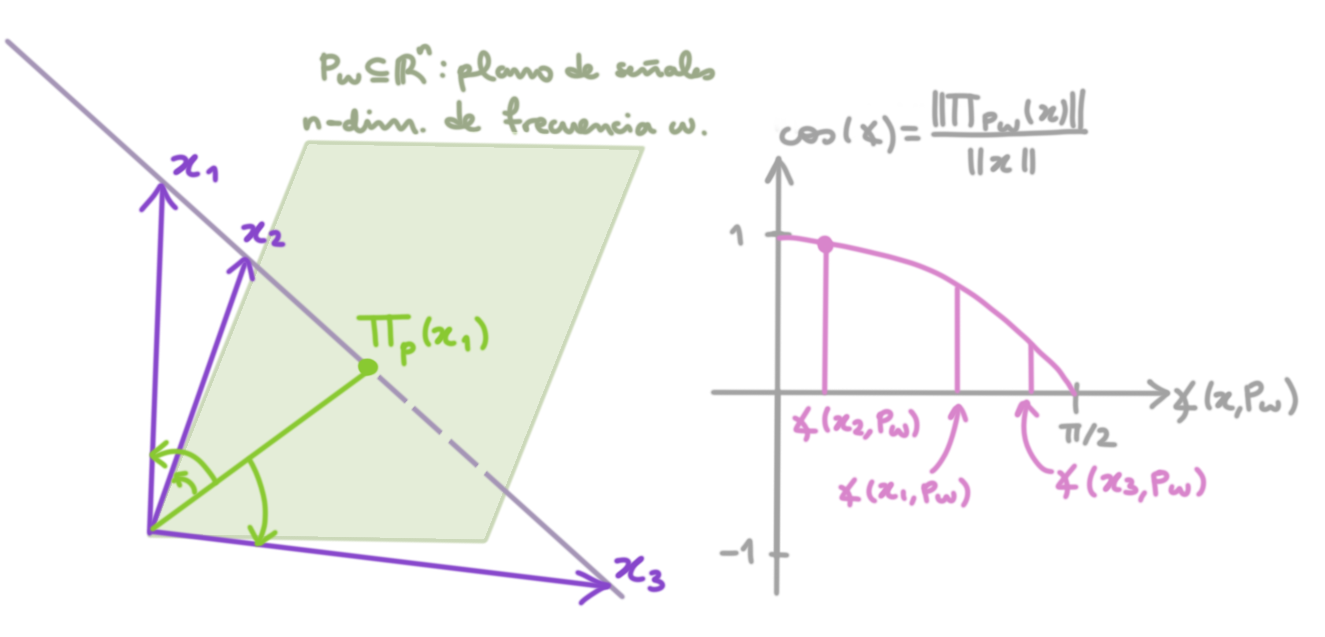
\includegraphics[scale= 1]{20Mar23_1} 
\end{figure}	

Puesto que todas las señales de Legendre discretas
$\mathcal{L}^{n,k}$ tienen norma uno,
\sidenote{En lo que resta de este capítulo, $x$ siempre denotará
a una señal unitaria.}
tenemos la relación simplificada 

\begin{equation}
\label{eq1: 20Mar}
cos \left( \measuredangle (x, W) \right) = || \Pi_{W}(x) || 
\hspace{0.5cm} (x \hspace{0.1cm} \text{unitario).}
\end{equation}

Para usar las fórmulas establecidas en 
la proposición \ref{prop: formulas 20Marzo}, debemos comprobar
que los vectores $f_{n, \omega}$ y $g_{n, \omega}$
son unitarios; hacemos esto, además de dar una fórmula
para su producto punto, en la siguiente proposición.


\begin{prop}
Fijados $n \geq 2$ y $\omega \geq 0$, los vectores
$f_{n, \omega}$ y $g_{n, \omega}$, como se definieron
en \eqref{eq5: 19Marzo}
y \eqref{eq6: 19Marzo}, respectivamente, 
son unitarios y linealmente independientes.
Además, 

\begin{equation}
\label{eq9: 19Marzo}
\langle f_{n, \omega} , g_{n, \omega} \rangle =
\frac{\xi_{n, w} \eta_{n, \omega}}{2} \cdot 
\frac{sen(2 \pi \omega)
sen(2 \pi \omega \left( 1- \frac{1}{n} \right))}{sen \left(2 \pi 
\frac{\omega}{n} \right)}
\end{equation}

\end{prop}
\noindent
\textbf{Demostración.}
El que los
vectores $f_{n, \omega}$ y $g_{n, \omega}$ sean ortogonales
se deduce del que la primera entrada de $f_{n, \omega}$ no sea cero
mientras que la primera entrada de $g_{n, \omega}$ sea cero, pero no
todas sus entradas sean cero. El que ambos vectores tengan norma
uno se deduce de unas operaciones análogas a las que realizaremos a
continuación para demostrar que en efecto se tiene la igualdad 
\eqref{eq9: 19Marzo}, por lo que omitiremos esos argumentos.


Aquí usaremos las siguientes tres igualdades:

\begin{equation}
\label{eq10: 19Marzo}
\forall \alpha \in \IR: \hspace{0.2cm}
sen(2 \alpha) = 2 sen(\alpha) cos(\alpha)
\end{equation}



\begin{equation}
\label{eq11: 19Marzo}
\forall z\in \IR: \hspace{0.2cm}
sen(z)= \frac{e^{iz}-e^{-iz}}{2i}
\end{equation}



\begin{equation}
\label{eq12: 19Marzo}
\forall a \in \IR-\{ 1 \}: \hspace{0.2cm}
\suma{\mu=0}{n-1}{a^{r}}= \frac{1-a^{n}}{1-a}.
\end{equation}


\begin{align*}
\langle f_{n,\omega} , g_{n, \omega} \rangle = &
\xi_{n, \omega} \eta_{n, \omega} \langle 
\left( cos (2 \pi \omega \frac{\mu }{n}) \right)_{0 \leq \mu \leq N-1} ,  
\left( cos (2 \pi \omega \frac{\mu }{n}) \right)_{0 \leq \mu \leq N-1} \rangle \\
= & \xi_{n, \omega} \eta_{n, \omega} \suma{\mu=0}{n-1}{
cos (2 \pi \omega \frac{\mu }{n}) sen(2 \pi \omega \frac{\mu }{n})} \\
= & \frac{\xi_{n, \omega} \eta_{n, \omega}}{2}
\suma{\mu=0}{n-1}{
\left( sen(4 \pi \omega \frac{\mu}{n}) \right)} \\
= & \frac{\xi_{n, \omega} \eta_{n, \omega}}{4i} \suma{\mu=0}{n-1}{
\left( e^{4 \pi \omega i \mu/n} - 
e^{-4 \pi \omega i \mu/n} \right) } \\
= & \frac{\xi_{n, \omega} \eta_{n, \omega}}{4i} 
\left(
\frac{1-e^{4 \pi \omega i }}{1-e^{4 \pi \omega i /N}} - 
\frac{1-e^{-4 \pi \omega i }}{1-e^{-4 \pi \omega i /N}} 
\right) \\
= & \frac{\xi_{n, \omega} \eta_{n, \omega}}{4i} 
\left(
\frac{e^{2 \pi \omega i }}{e^{2 \pi \omega i/n }}
\frac{e^{-2 \pi \omega i }-e^{2 \pi \omega i }}{e^{-2 \pi \omega i/n }-e^{2 \pi \omega i /N}} - 
\frac{e^{-2 \pi \omega i }}{e^{-2 \pi \omega i/n }}
\frac{e^{2 \pi \omega i }-e^{-2 \pi \omega i }}{e^{2 \pi \omega i/n }-e^{2 \pi \omega i /N}} 
\right) \\
= & 
\frac{\xi_{n, \omega} \eta_{n, \omega}}{4i} 
\left(
e^{2 \pi \omega i \left( 1-1/n \right)}
\frac{sen(2 \pi \omega)}{sen(2 \pi \omega /n)} - 
e^{-2 \pi \omega i \left( 1-1/n \right)}
\frac{sen(2 \pi \omega)}{sen(2 \pi \omega /n)}
\right) 
\\
= & 
\frac{\xi_{n, \omega} \eta_{n, \omega}}{4i} 
\frac{sen(2 \pi \omega)}{sen(2 \pi \omega /n)}
\left(
e^{2 \pi \omega i \left( 1-1/n \right)} - e^{-2 \pi \omega i \left( 1-1/n \right)}
\right) \\
= &
\frac{\xi_{n, \omega} \eta_{n, \omega}}{4i} 
\frac{sen(2 \pi \omega)}{sen(2 \pi \omega /n)}
\left(
2i \cdot  sen \left( 2 \pi \omega  \left( 1- \frac{1}{n} \right) \right)
\right)\\
= & 
\frac{\xi_{n, \omega} \eta_{n, \omega}}{2} 
\frac{sen(2 \pi \omega)}{sen(2 \pi \omega /n)}
sen \left( 2 \pi \omega  \left( 1- \frac{1}{n} \right) \right). \\
\end{align*}


\QEDB
\vspace{0.2cm}


Podemos ya usar la
fórmula \eqref{eq3: 19Marzo} en nuestra situación particular para llegar a que

\[
|| \Pi_{P}(x) ||=
		\left(		  
		  \frac{1}{1- \langle f_{n, \omega }, g_{n, \omega } \rangle^{2}} \left(  
	       \langle x, f_{n, \omega } \rangle^{2} +  \langle x, g_{n, \omega } \rangle^{2}	
	       -2  \langle x, f_{n, \omega } \rangle^{2} \langle x, g_{n, \omega } \rangle^{2} \langle f_{n, \omega }, g_{n, \omega } \rangle^{2}	  
		  \right)
		  \right) ^{1/2}
\]

\TODO{Di que estas son las nuevas sigmas que graficas.}

\subsection{Buscando el mejor desfase con cierta frecuencia que se ajuste una señal de dimensión $n$}

Dada $x \in \IR^{n}$ unitaria y $\omega > 0$ una frecuencia fija, 
buscamos el desfase $\phi \in [0,1]$ que mejor se ajusta a $x$; puesto que
$\Pi_{P_{\omega}}(x)$ (donde $P_{\omega}$ es como se definió en 
\eqref{eq2: 20Marzo}) es la señal de frecuencia $\omega$ que está a menor
distancia euclidea de $x$, claro que el desfase $\phi$ buscado es de hecho
el número entre cero y uno tal que 
\[
\Pi_{P_{\omega}}(x) = \alpha (cos(2 \pi \omega (t - \phi)))_{t \in I_{n}}
\]
para alguna amplitud $\alpha$.

La ecuación \eqref en nuestro contexto se reescribe como

\begin{equation}
\label{eq3: 20Marzo}
\Pi_{P_{\omega}}(x)= c (cos (2 \pi \omega t))_{t \in I_{n}} + d 
(sin (2 \pi \omega t))_{t \in I_{n}},
\end{equation}
donde

\begin{equation}
\label{eq4: 20Marzo}
c= \frac{
\langle x, f_{n, \omega} \rangle - \langle f_{n, \omega}, g_{n, \omega} \rangle
\langle x, g_{n, \omega} \rangle
}{1-\langle f_{n, \omega}, g_{n, \omega} \rangle^{2}} \xi_{n, \omega}
\end{equation}
y
\begin{equation}
\label{eq5: 20Marzo}
d= \frac{
\langle x, g_{n, \omega} \rangle - \langle f_{n, \omega}, g_{n, \omega} \rangle
\langle x, f_{n, \omega} \rangle
}{1-\langle f_{n, \omega}, g_{n, \omega} \rangle^{2}} \eta_{n, \omega}.
\end{equation}

Nos conviene más reescribir a \eqref{eq3: 20Marzo} como
\begin{equation}
\label{eq6: 20Marzo}
\Pi_{P_{\omega}}(x)= 
\sqrt{c^{2}+d^{2}}
\left(
C (cos (2 \pi \omega t))_{t \in I_{n}} +
D (sen (2 \pi \omega t))_{t \in I_{n}} 
\right),
\end{equation}

donde
\[
C:= \frac{c}{\sqrt{c^{2}+d^{2}}}
\]
y 
\[
D:= \frac{d}{\sqrt{c^{2}+d^{2}}},
\]
pues, como $C^{2} + D^{2}=1$, existe un único
$\phi \in [0,1]$ (\TODO{mejor cámbiale el nombre}) tal que
\begin{equation}
\label{eq7: 20Marzo}
C= cos(2 \pi \phi), \hspace{0.2cm} 
D= sin(2 \pi \phi).
\end{equation}

Sustituyendo \eqref{eq7: 20Marzo} en \eqref{eq6: 20Marzo},
llegamos a que

\begin{align*}
\Pi_{P_{\omega}}(x) = & 
\sqrt{c^{2}+d^{2}} \left(
cos(2 \pi \phi) \cdot (cos (2 \pi \omega t))_{t \in I_{n}} +
sin(2 \pi \phi) \cdot (sin (2 \pi \omega t))_{t \in I_{n}} 
\right) \\
= & 
\sqrt{c^{2}+d^{2}} 
((cos(2 \pi \phi) \cdot cos (2 \pi \omega t) +
sin(2 \pi \phi) \cdot sin (2 \pi \omega t) )_{t \in I_{n}} \\
= & 
\sqrt{c^{2}+d^{2}} 
\left(
cos \left( 2 \pi \omega \left( t - \frac{\phi}{\omega}
\right) 
\right) 
\right)_{t \in I_{n}}
\end{align*}